%
%  Austin Powell
%
\documentclass[12pt,fullpage]{article}
\usepackage{fullpage}
\usepackage{psfrag}                                          % LaTeX graphics tool
\usepackage{pslatex}                                         % avoids the default cmr font
\usepackage{graphicx}                                        % graphics package 
\usepackage{epsfig} 
\usepackage{hyperref}
\usepackage{color}

\begin{document}

\noindent
{\bf Laplace distribution} (from \color{blue}\url{http://www.math.wm.edu/~leemis/chart/UDR/UDR.html}\color{black})

\noindent
The shorthand $X \sim {\rm Laplace}(\alpha_1, \, \alpha_2)$ is used to indicate
that the random variable $X$ has the Laplace distribution with
positive scale parameters $\alpha_1$ and $\alpha_2$. A Laplace random variable $X$ has probability density function
$$
f(x) = \left\{ \begin{array}{ll}
(1/(\alpha_1 + \alpha_2))e^{\kern 0.04em x/\alpha_1} & \qquad x < 0 \\
(1/(\alpha_1 + \alpha_2))e^{-x/\alpha_2} & \qquad x \geq 0
\end{array}
\right.
$$
for $\alpha_1, \alpha_2 > 0$.
The Laplace distribution is an alternative to the normal distribution with heavier tails.
The probability density function for three different parameter settings is illustrated below.

\begin{figure}[h!]
\begin{center}
\psfrag{laba11}{$\alpha_1 = 1$}
\psfrag{laba21}{$\alpha_2 = 1$}
\psfrag{laba12}{$\alpha_1 = 2$}
\psfrag{laba22}{$\alpha_2 = 2$}
\psfrag{labf}{$f(x)$}
\includegraphics[width=5.2in]{LaplacePlot.ps}
\end{center}
\end{figure}

\noindent
The cumulative distribution function on
the support of $X$ is
$$
F(x) = P (X \leq x) = \left\{ \begin{array}{ll}
(\alpha_1/(\alpha_1 + \alpha_2))e^{\kern 0.04em x/\alpha_1} & \qquad x < 0 \\
1 - (\alpha_2/(\alpha_1 + \alpha_2))e^{-x/\alpha_2} & \qquad x \geq 0.
\end{array}
\right.
$$
The survivor function on the support of $X$ is
$$
S(x) = P (X \geq x) = \left\{ \begin{array}{ll}
1 - (\alpha_1/(\alpha_1 + \alpha_2))e^{\kern 0.04em x/\alpha_1} & \qquad x < 0 \\
(\alpha_2/(\alpha_1 + \alpha_2))e^{-x/\alpha_2} & \qquad x \geq 0.
\end{array}
\right.
$$
The hazard function on the support of $X$ is
$$
h(x) = \frac{f(x)}{S(x)} = \left\{ \begin{array}{ll}
e^{\kern 0.04em x/\alpha_1}/(\alpha_1 + \alpha_2 + \alpha_1 e^{\kern 0.04em x/\alpha_1}) & \qquad x < 0 \\
1/\alpha_2 & \qquad x \geq 0.
\end{array}
\right.
$$
The inverse distribution function of $X$ is
$$
F ^ {-1}(u) = \left\{ \begin{array}{ll}
-\alpha_1\left(-\ln(\alpha_1 + \alpha_2) + \ln(\alpha_1) - \ln(u)\right) & \qquad 0 < u < \alpha_1/(\alpha_1 + \alpha_2) \\
-\alpha_2\left(\ln(\alpha_1 + \alpha_2) - \ln(\alpha_2) + \ln(1 - u)\right) & \qquad \alpha_1/(\alpha_1 + \alpha_2) \leq u < 1.
\end{array}
\right.
$$
The moment generating function and the characteristic function of $X$ are mathematically intractable.

\vspace{0.1in}
\noindent
The population mean, variance, skewness, and kurtosis of $X$ are
$$
E[X] = \alpha_2 - \alpha_1 \qquad \qquad 
V[X] = \alpha_1^2 + \alpha_2^2 \qquad \qquad
$$
$$
E\left[ \left( \frac{X - \mu}{\sigma} \right)^3 \right] = - \frac{2(\alpha_1^3 - \alpha_2^3)}{(\alpha_1^2 + \alpha_2^2)^{3/2}}  \qquad \qquad
E\left[ \left( \frac{X - \mu}{\sigma} \right)^4 \right] = \frac{3(3\alpha_1^4 + 2\alpha_2^2 \alpha_1^2 + 3\alpha_2^4)}{(\alpha_1^2 + \alpha_2^2)^2}.
$$

\vspace{0.1in}

\noindent
{\bf APPL verification:}
The APPL statements
\begin{verbatim}
assume(alpha1 > 0);
assume(alpha2 > 0);
X := [[x -> exp(x / alpha1)/(alpha1 + alpha2),
       x -> exp(-x / alpha2)/(alpha1 + alpha2) ],
       [-infinity, 0, infinity], ["Continuous", "PDF"]]; 
CDF(X);
SF(X);
HF(X);
IDF(X);
Mean(X);
Variance(X);
Skewness(X);
Kurtosis(X);
\end{verbatim}
verify the cumulative distribution function, survivor function, hazard function, population mean, variance, skewness, and kurtosis.
\end{document}
